\chapter{Week}
At the beginning of the week a task unrelated to \ac{AI} was given to check upon internal documentation and customer support. Together with another recently hired employee, a day of out-of-box testing was scheduled. An Enclustra base board (Mercury+ PE1-400) together with a fitting \ac{FPGA} module (Mercury+ XU1) featuring a Xilinx \ac{MPSoC}.
Some details will be given for this specific \ac{FPGA} family as the Zynq-7000 \ac{SoC} and the Zynq-\ac{MPSoC} Xilinx product family are unique in the way dedicated ARM processors are combined with traditional \acp{FPGA}. A high level overview is shown in figure~\ref{fig:zynq-overview}.
\begin{figure}[!htb]
	\centering
		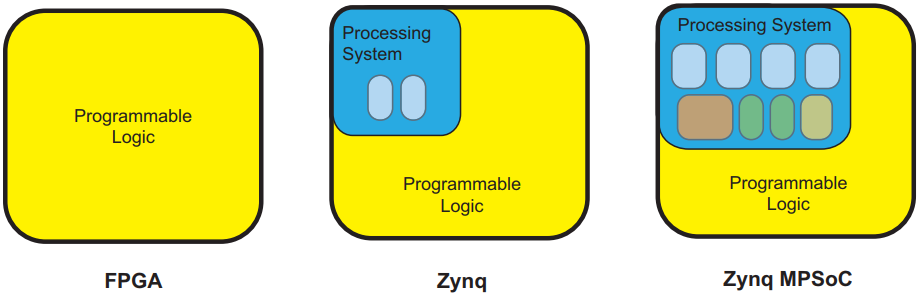
\includegraphics[width=\textwidth]{bilder/ZYNQ-overview.png}
		\caption{High level ZYNQ family overview~\cite{zynq-book}}
		\label{fig:zynq-overview}
\end{figure}
It shows the difference between traditional \acp{FPGA} and the Zynq product family. The main benefit here is the division between \ac{PS} and \ac{PL}. This allows to combine the benefits of traditional processing units with the flexibility of \acp{FPGA}. Custom logic and all peripheral devices can be implemented in the \ac{PL} part, while system control and even complete \acp{OS} (such as embedded Linux) can be done in the \ac{PS}. As this system is completely integrated in one package, the communication between the two fabrics is extremely fast and can be done using \ac{AXI} interfaces. The \ac{MPSoC} family even integrates several different types of processing units, \acp{APU}, \acp{GPU}, \acp{VPU} and \acp{RPU}.
The Enclustra module uses an \ac{MPSoC} Xilinx FPGA and our task was to go through the whole process of bringing up the base board together with a corresponding module to test customer experience using the provided documentation, user manual and reference design. The goal was to find unclear instructions in the documentation and provide feedback as to the overall experience bringing up the hardware out-of-the-box. First, the hardware reference design was loaded in the Vivado Design Suite and the bit stream generated. After, the hardware description file was exported so it can be used using the Xilinx \ac{SDK}. This allows to create applications in C/C++ against the custom hardware design. All of the provided sample applications have been tested and verified. Some unclear instructions were identified and discussed with the employee in charge to improve customer experience.
The rest of the week was spend updating the internal Wiki page for \ac{AI}. Furthermore, the \ac{DNNDK} sample applications were tested on the ZCU 104 evaluation board. The provided examples include several state-of-the-art neural networks demonstrating key applications for neural network inference, such as image classification, face detection, object detection and pose detection. As only the image classification example worked directly for this particular evaluation a fix needed to be found. Another task was to introduce the topic of \ac{AI} to the whole company as \acp{ANN} was a completely new design field for a majority of the technical staff. Two PowerPoint presentations should be prepared, namely 'Introduction to \ac{AI}' and 'Introduction to \ac{ML} on \acp{FPGA}'. I started with the preparation of the first one in parallel with finding a bug fix for the other \ac{DNNDK} sample applications, as these should be part of the second presentation.